\documentclass{../template/texnote}

\title{Contour Plot}

\begin{document}
    \maketitle \currentdoc{note}
    %<*note>

\section{Contour plots}
URL: \url{https://www.youtube.com/watch?v=ImeCXBQtx6k}

A contour plot in two dimensions are the isolines of a scalar field that depends on two variables.
Figure \ref{fig:contour_demo} shows the contour plot for the function
$Z = \sin{X} + \cos{Y}$.
\begin{figure}
\begin{center}
    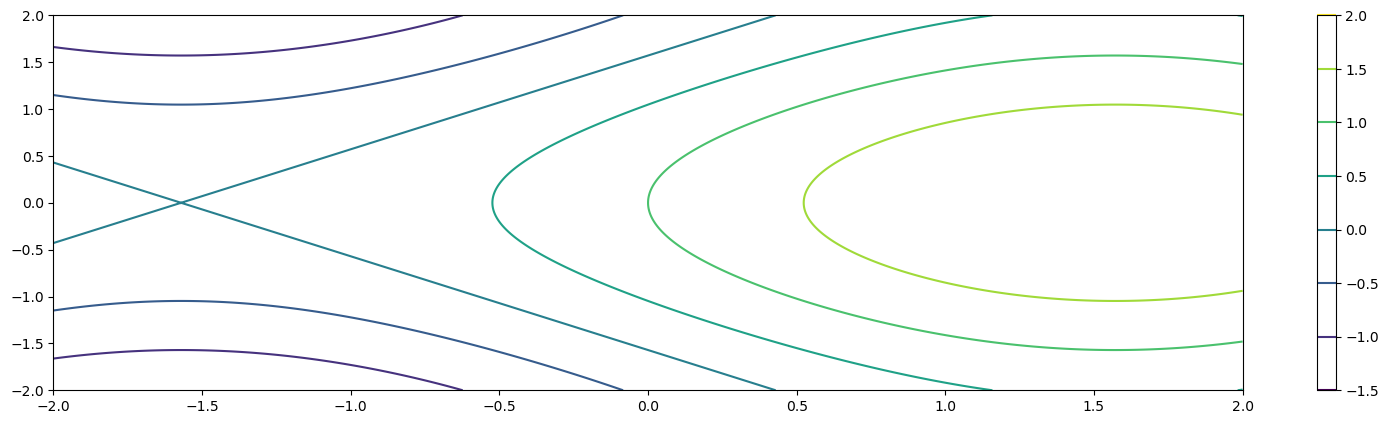
\includegraphics[width=1.2\linewidth]{contour_demo.png}
\end{center}
\caption{A demo contour plot}
\label{fig:contour_demo}
\end{figure}
If more levels are specified we get Figure \ref{fig:contour_levels}.
\begin{figure}
\begin{center}
    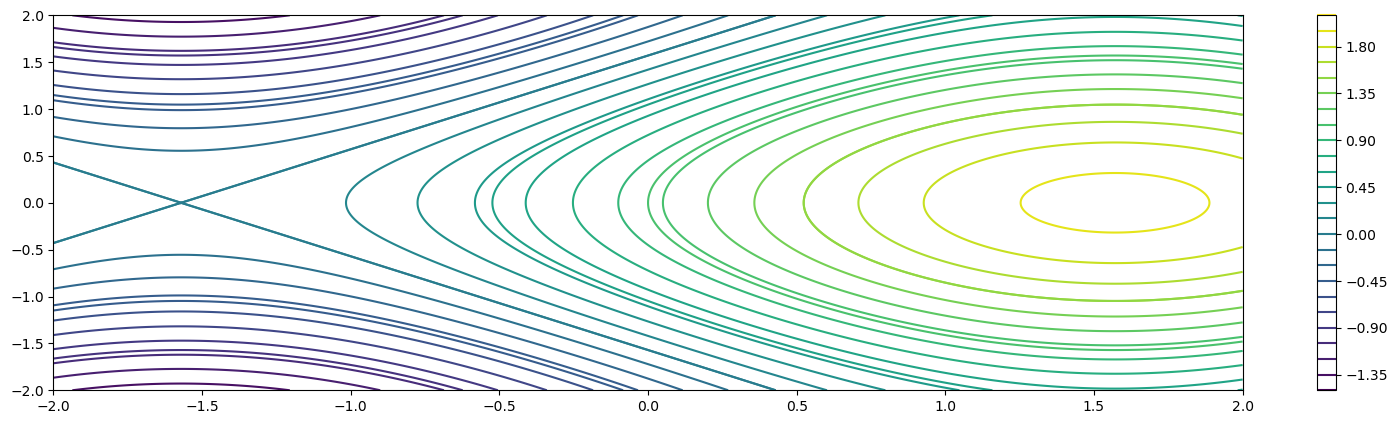
\includegraphics[width=1.2\linewidth]{contour_demo_levels.png}
\end{center}
\caption{contour plot with 30 levels specified}
\label{fig:contour_levels}
\end{figure}


    %</note>
    \printbibliography
\end{document}
